%% Prof. Ed Merkle, University of Missouri
%% Charlie Redmon, University of Kansas
%% 20170918
%% SEM path diagram

% standalone class for individual image to be included in a document
% border=15pt controls the whitespace padding around the diagram
\documentclass[border=15pt]{standalone}

% load custom style configurations from separate file
%% ------------------------------------------------------------
%% Charlie Redmon
%% 20170923
%% semTikzStyle.tex: style configurations for SEM path diagrams
%% ------------------------------------------------------------

\usepackage{tikz}

% observed variable
\tikzstyle{ov}=[shape=rectangle,
                draw=black!80,
                minimum height=0.6cm,
                minimum width=0.6cm,
                thick]

% response variable
\tikzstyle{av}=[shape=rectangle,
                draw=black!80,
                fill=black!10,
                minimum height=0.6cm,
                minimum width=0.6cm,
                thick]

% latent variable
\tikzstyle{lv}=[shape=circle,
                draw=black!80,
                thick,
                minimum width=1cm]

% correlations
\tikzstyle{lcor}=[bend left=30, dashed]
\tikzstyle{rcor}=[bend right=30, dashed]

% self-loops (for variance)
\tikzstyle{lloop}=[loop left, 
                   out=210, 
                   in=150, 
                   distance=0.3cm,
                   densely dotted]

\tikzstyle{rloop}=[loop right, 
                   out=30, 
                   in=-30, 
                   distance=0.3cm,
                   densely dotted]

\tikzstyle{aloop}=[loop above, 
                   out=60, 
                   in=120, 
                   distance=0.3cm,
                   densely dotted]

\tikzstyle{bloop}=[loop below, 
                   out=-60, 
                   in=-120, 
                   distance=0.3cm,
                   densely dotted]




\begin{document}

%% ">=stealth" sets the arrow head style
%% "semithick" sets the line width (0.6 pt)
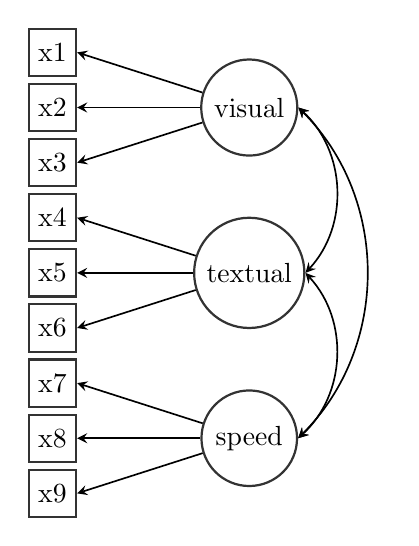
\begin{tikzpicture}[>=stealth,semithick,scale=0.5]

% observed variables
\node[ov] (y1) at (0,0)  {x1};
\node[ov] (y2) at (0,-1.4)  {x2};
\node[ov] (y3) at (0,-2.8)  {x3};
\node[ov] (y4) at (0,-4.2)  {x4};
\node[ov] (y5) at (0,-5.6)  {x5};
\node[ov] (y6) at (0,-7)  {x6};
\node[ov] (y7) at (0,-8.4)  {x7};
\node[ov] (y8) at (0,-9.8)  {x8};
\node[ov] (y9) at (0,-11.2)  {x9};

% latent variables
\node[lv] (f1) at (5, -1.4)  {visual};
\node[lv] (f2) at (5, -5.6)  {textual};
\node[lv] (f3) at (5, -9.8)  {speed};

% paths
\path[->] (f1) edge node[above=0.08cm,scale=0.8,pos=0.7] {} (y1.east);
\path[->] (f1) edge node[above=0.08cm,scale=0.8,pos=0.7] {} (y2.east);
\path[->] (f1) edge node[above=0.08cm,scale=0.8,pos=0.7] {} (y3.east);
\path[->] (f2) edge node[above=0.08cm,scale=0.8,pos=0.7] {} (y4.east);
\path[->] (f2) edge node[above=0.08cm,scale=0.8,pos=0.7] {} (y5.east);
\path[->] (f2) edge node[above=0.08cm,scale=0.8,pos=0.7] {} (y6.east);
\path[->] (f3) edge node[above=0.08cm,scale=0.8,pos=0.7] {} (y7.east);
\path[->] (f3) edge node[above=0.08cm,scale=0.8,pos=0.7] {} (y8.east);
\path[->] (f3) edge node[above=0.08cm,scale=0.8,pos=0.7] {} (y9.east);

% paths between latent variables
\path[<->] (f1.east) edge [bend left=45] node[left,scale=0.8] {} (f2.east);
\path[<->] (f1.east) edge [bend left=45] node[left,scale=0.8] {} (f3.east);
\path[<->] (f2.east) edge [bend left=45] node[left,scale=0.8] {} (f3.east);

\end{tikzpicture}



\end{document}